\chapter{Simulations}
\label{chap:simulations}

\section{SNAP library}
\label{section:snap}
In order to run the simulations necessary to validate the project, a robust library was required to handle graph data structures.
The Stanford Network Analysis Platform (SNAP) library \cite{snap} was chosen primarily because it is memory efficient.
The simulations require multiple graphs that share the same set of nodes (because each node in the network has its own knowledge of the surrounding network), and the SNAP library uses pointers to nodes and edges, saving memory by not having to duplicate the entire data structure.
It is written in C++, but, for these simulations, the Snap.py Python library was used.

%The datasets available from SNAP's website were used for the simulations in \cite{vernize2015malicious} and the static network simulations shown in \autoref{chap:simulations}.

\section{The ONE Simulator}
\label{section:theone}

\section{Working Day Movement Model}
\label{section:workingday}

Most VANET trust models consider the Random Waypoint mobility model, i.e. each node has an origin point, chooses a random location, gets to that location, then chooses another random location and goes there, and so forth.
While this model is efficient for testing trust protocols, it doesn't truly represent vehicle mobility in the real world.

To make use of the properties described in \autoref{section:socialvanets}, it is important to choose a mobility pattern that properly represents the way vehicles move on a daily basis in the real world.
Therefore, the Working Day Movement Model \cite{ekman2008working} (WDM) is useful.
The model, developed for use in Delay-Tolerant Network (DTN) simulations, includes many of the features that are necessary to simulate the daily movement of a vehicular network.

As the name implies, the Working Day Model abstracts people's movement from their homes to their offices and back.
Each node has a home and a workplace and they need to travel back and forth between those locations on a daily basis.
Occasionally, nodes can also go to other locations for leisure.
As mentioned above, many drivers have routes they travel on daily, so the Working Day model is a more accurate representation, although it represents the mobility of humans instead of vehicle and requires some adjustments, which are listed later in this section.

The model proposed by the authors makes use of several other models for specific tasks.
The main mobility model defines nodes and gives them their destinations.
Within it, five other models are used:
\begin{enumerate}
\item 
The \textbf{home activity submodel} describes what nodes do at night, within their homes.
No movement is modeled.
Nodes can be relatives or neighbors, and therefore share the same home.
\item 
The \textbf{office activity submodel} describes the nodes' routines within their offices.
Nodes can go to other locations within the office (such as meeting rooms) and such movement is modeled.
Nodes with share the same office are coworkers.
\item 
The \textbf{evening activity submodel} is responsible for mobility outside the nodes' standard routine. 
They can meet at certain locations (such as restaurants) and spend a few hours gathered with friends.
\item
The \textbf{transport submodel} shows how nodes move around the city.
It includes another tier of submodels, responsible for modeling three different types of transportation: walking, driving, and riding a bus.
Nodes which own a car always use it, while the others can decide to walk or ride a bus depending on the distance between the origin and destination and the available bus stops.
The walking and driving submodels represent similar types of movement, although at different speeds, while the bus submodel follows cyclical routes and can take or deliver passengers at bus stops.
\item
The \textbf{map} represents the city in which the simulation runs.
Its streets constrain the movement of nodes and all homes and offices must be within the map boundaries.
The map can be divided into districts, which increases what the authors define as \textit{locality}.
In the simulation parameters, the number of nodes which reside and work within the same district can be chosen, which means those nodes rarely leave the district.
Nodes which reside and work in different districts serve to connect the network with their commutes.
\end{enumerate}

By thinking of these submodels for vehicles instead of people, it can become apparent how the frequency and length of encounters between nodes are similar in both instances.
If two vehicles belong to family members or neighbors, they likely spend most of the night within communication distance, while coworkers' cars spend the office hours close by.
Cars can also meet each other frequently if their drivers go out with friends.
In the vehicular case, there is the added layer of encounters: cars can communicate frequently with buses and other cars that take the same route daily, although the drivers are likely complete strangers.

In the original article, nodes are devices (such as smartphones) being carried by humans.
Therefore, the Working Day model represents not only people's movements inside their cars, but also within their offices, walking on foot, or riding a bus.
To adapt it to a VANET environment, changes need to be made to their definition of node, since they now represent vehicles instead of people. Some of those changes are as follows:
\begin{enumerate}
\item
The office activity submodel no longer needs to model movement within the office and can be identical to the home submodel.
In both, a node can move a small amount once after reaching the office or home, to simulate parking.
This can be done using the Working Day model's parameters.
\item
The walking submodel needs to be disabled, since all nodes are either cars or buses.
\item
The bus submodel needs to be changed so that each bus is one node in the network, which follows a predefined route with bus stops.
In the original model, each bus could carry several nodes, but this is no longer necessary.
\end{enumerate}
Other necessary changes might become apparent during the development of the study.

One important topic raised in the Working Day movement model article is the use of two metrics: \textit{inter-contact times} and \textit{contact duration}.
The choice of this movement model for tests is more strongly related to inter-contact times, i.e. how much time it takes for two nodes to meet again.
On the other hand, the contact duration is how long each meeting lasts.
For the reasons explained earlier in this section, relatively short inter-contact times is important for the proposed trust model.
Contact duration time is an important metric to measure how much data can be exchanged during each encounter, although taking it into consideration might add excessive complexity to the model.

\section{Simulation parameters and methodology}
\label{section:parameters}

In order to test the TruMan trust model, simulations were made using an implementation of the algorithm in Python.
To generate the input graphs with node mobility, the ONE simulator \cite{keranen2009one} was used in conjunction with the Working Day Movement Model \cite{ekman2008working}, which provides a strong similarity with vehicle movement in real life.
Snapshots of the network were taken every 10 simulated seconds, and these snapshots were used as input for the algorithm.

\begin{table}[h!]
\caption{Simulation parameters}
\label{table:parameters}
\centering
\begin{tabular}{|p{5cm}||p{5cm}|}
 \hline
 \textbf{Parameter}	& \textbf{Value} \\
 \hline
 \hline
 Duration 			& 86400 seconds \\
 \hline
 Work day length 	& 28800 seconds \\
 \hline
 Std. dev. departure time & 7200 seconds \\
 \hline
 Node velocity 		& 7~10m/s \\
 \hline
 Simulation area	& approximately 14km\textsuperscript{2} \\
 \hline
 Number of nodes 	& 150 (WDMM) + 10 (random) \\
 \hline
% Cost & O(|V|* |E|) & O(|V|+|E|) & n/a & n/a & n/a \\
% \hline
\end{tabular}
\end{table}

Most of the parameters for the simulator were taken from the article detailing the Working Day Movement Model \cite{ekman2008working}.
Different parameters are shown in \autoref{table:parameters}.
The simulation ran for 86400 seconds (24 hours), with a work day length of 28800 seconds and a standard deviation of departure time of 7200 seconds.
Nodes move between 7 and 10 m/s in an area of approximately 14 km\textsuperscript{2} based on a section of the map of Helsinki.
%The number of nodes and their communication range vary for different simulations.
There is a total of 160 nodes, 150 of which are following the Working Day Movement Model, and the other 10 are moving randomly to simulate vehicles that do not follow daily patterns.
Since this simulation is for vehicles instead of pedestrians, there are no buses in the model and every node is guaranteed to own a vehicle and travel by car.
The parameters regarding offices, meeting spots and shopping were kept intact.
A small part of nodes move randomly to simulate vehicles that do not follow daily patterns.

\subsection{Network Density}

%==> PRECISA MOSTRAR A EQUAÇÃO DE CALCULO DA DENSIDADE, SENÃO FICA DIFICIL DE ENTENDER O CALCULO.

The communication range of nodes varies from 10m to 50m, to illustrate the impact of different network densities.
The network density ($\delta$) is a value which abstracts the volume and frequency of connections in a vehicular network by estimating how much of the environment is covered by the network.
For TruMan, higher densities yield better results, since nodes can construct and update their models of the network faster (this is demonstrated in \autoref{subsection:simulations}).
It is calculated using the transmission range of the nodes ($\rho$), the amount of nodes ($\eta$), and the total area of the simulation ($\alpha$).

The coverage of a single node is the circumference around it formed by the transmission radius. This is divided by two to compensate for overlapping circumferences, then multiplied by the number of nodes in the network to estimate the maximum coverage area.
Finally, the value is divided by the total area of the environment.
The network density formula is as follows:

$$ \delta = \frac{\frac{\rho^2\pi}{2} \times \eta}{\alpha} $$

Simulations shown here have densities between 0.001 ($\rho = 10$m) and 0.04 ($\rho = 50$m).
As a comparison, the density of the city of São Paulo (Brazil) was calculated as 2.24 with $\rho = 10$m, a much higher value than what is necessary for a satisfactory performance of the algorithm.

\subsection{Validation}

\section{Restrictions}
\label{section:restrictions}

\section{Results}
\label{section:results}

To improve readability, all figures in this section follow the same format:
$X$ axis shows the results of sequential iterations, ranging from 0 to 8639;
$Y$ axis shows a percentage of all nodes in the network, ranging from 0 to 100;
blue line represents the percentage of nodes detected out of the complete network;
magenta is the percentage of malicious nodes in the network (ground truth);
green represents the nodes correctly identified as malicious (true positives);
cyan represents the undetected malicious nodes (false negatives); 
red represents the benign nodes incorrectly identified as malicious (false positives).

\autoref{fig:random103050} shows the results of simulations running with 10\% of nodes acting maliciously, with communications range varying from 10m to 50m.
It is possible to see how the increase in the range allows the algorithm to converge sooner, taking over 8000 iterations with 10m range and achieving solid results at just over 1000 iterations with 50m range. 

\autoref{fig:random0} shows the variation of results for different amounts of malicious nodes in the network.
By the end of one day, the algorithm is able to detect all malicious nodes when they are up to 30\% of the network.
At 40\%, a small part of malicious nodes are yet to be detected.
At 50\%, as expected, the results are inconsistent as the network is completely split between benign and malicious nodes; at this point, the network is completely compromised.
The amount of malicious nodes also affects the convergence of the algorithm, since nodes do not trust information from malicious neighbors.

\autoref{fig:random7} shows the execution of the algorithm over the course of 7 days.
Most malicious nodes are identified by the end of the first day; in the following iterations, the algorithm finishes building the network model and sorts out remaining false negative or false positive results.
After iteration 20000, the results are completely consistent.

\begin{figure}
\centering

\begin{subfigure}{0.5\textwidth}
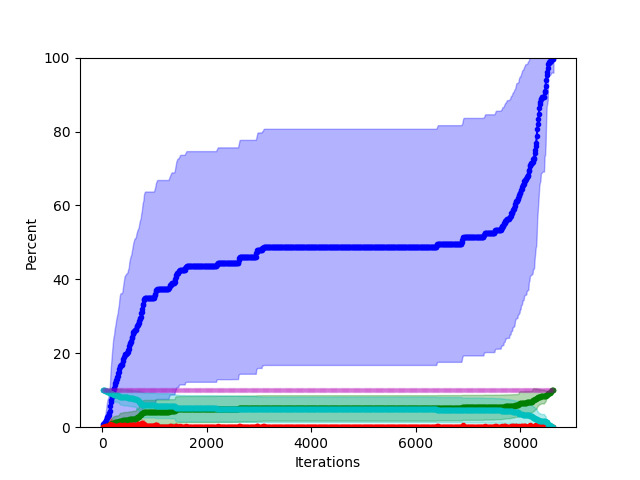
\includegraphics[width=\linewidth]{images/plots/Network_rA_10.0/new_plots/10.png}
\caption{$\rho$ = 10m.} \label{fig:tarjan0}
\end{subfigure}

\begin{subfigure}{0.5\textwidth}
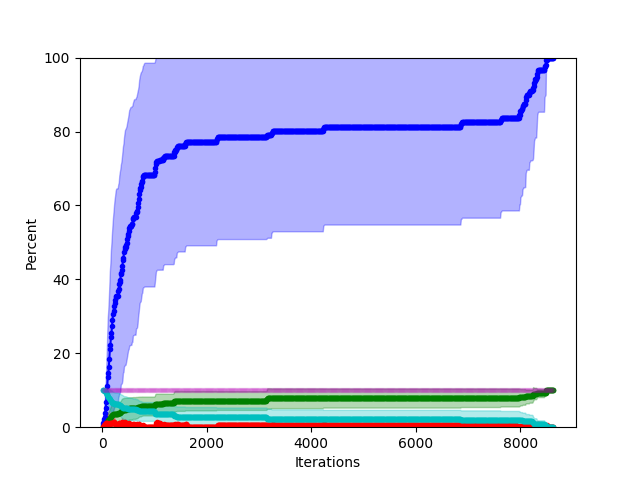
\includegraphics[width=\linewidth]{images/plots/Network_rA_10.0/new_plots/30.png}
\caption{$\rho$ = 30m.} \label{fig:tarjan0}
\end{subfigure}

\begin{subfigure}{0.5\textwidth}
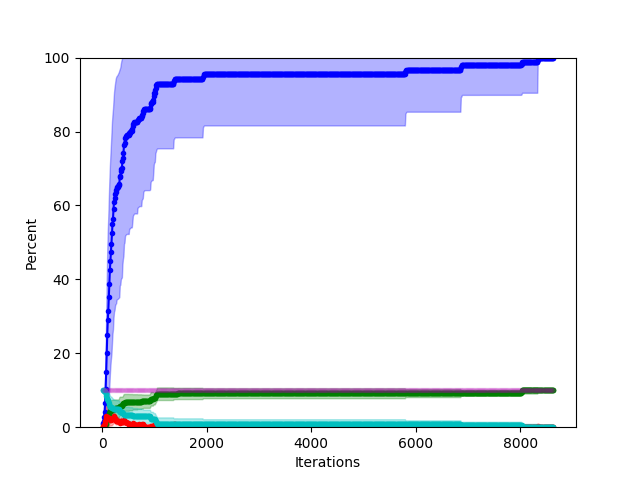
\includegraphics[width=\linewidth]{images/plots/Network_rA_10.0/new_plots/50.png}
\caption{$\rho$ = 50m.} \label{fig:tarjan0}
\end{subfigure}

\caption{Simulation with 10\% malicious nodes and varying values of $\rho$.}
\label{fig:random103050}
\end{figure}



\begin{figure}
\centering

\begin{subfigure}{0.45\textwidth}
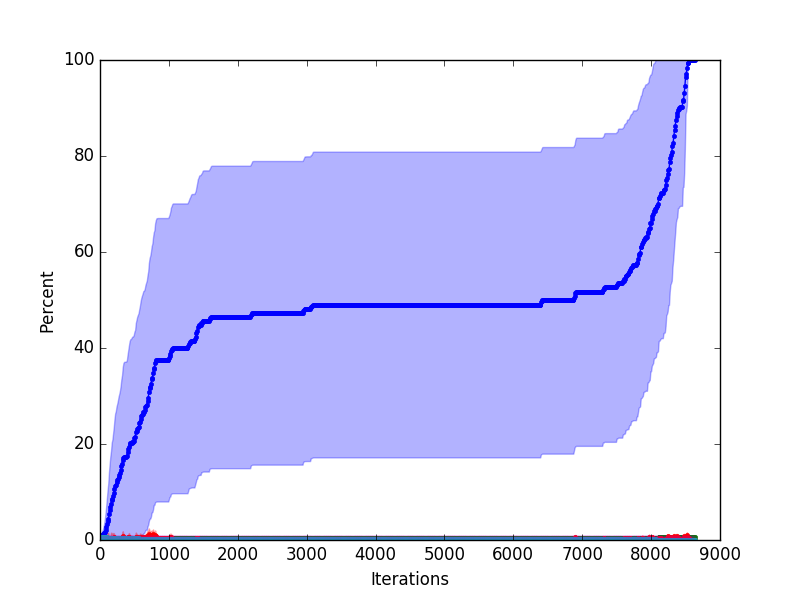
\includegraphics[width=\linewidth]{images/plots/Network_rA/10_1.png}
\caption{1\% malicious.}
\end{subfigure}
\hspace*{0.1cm} % separation between the subfigures
\begin{subfigure}{0.45\textwidth}
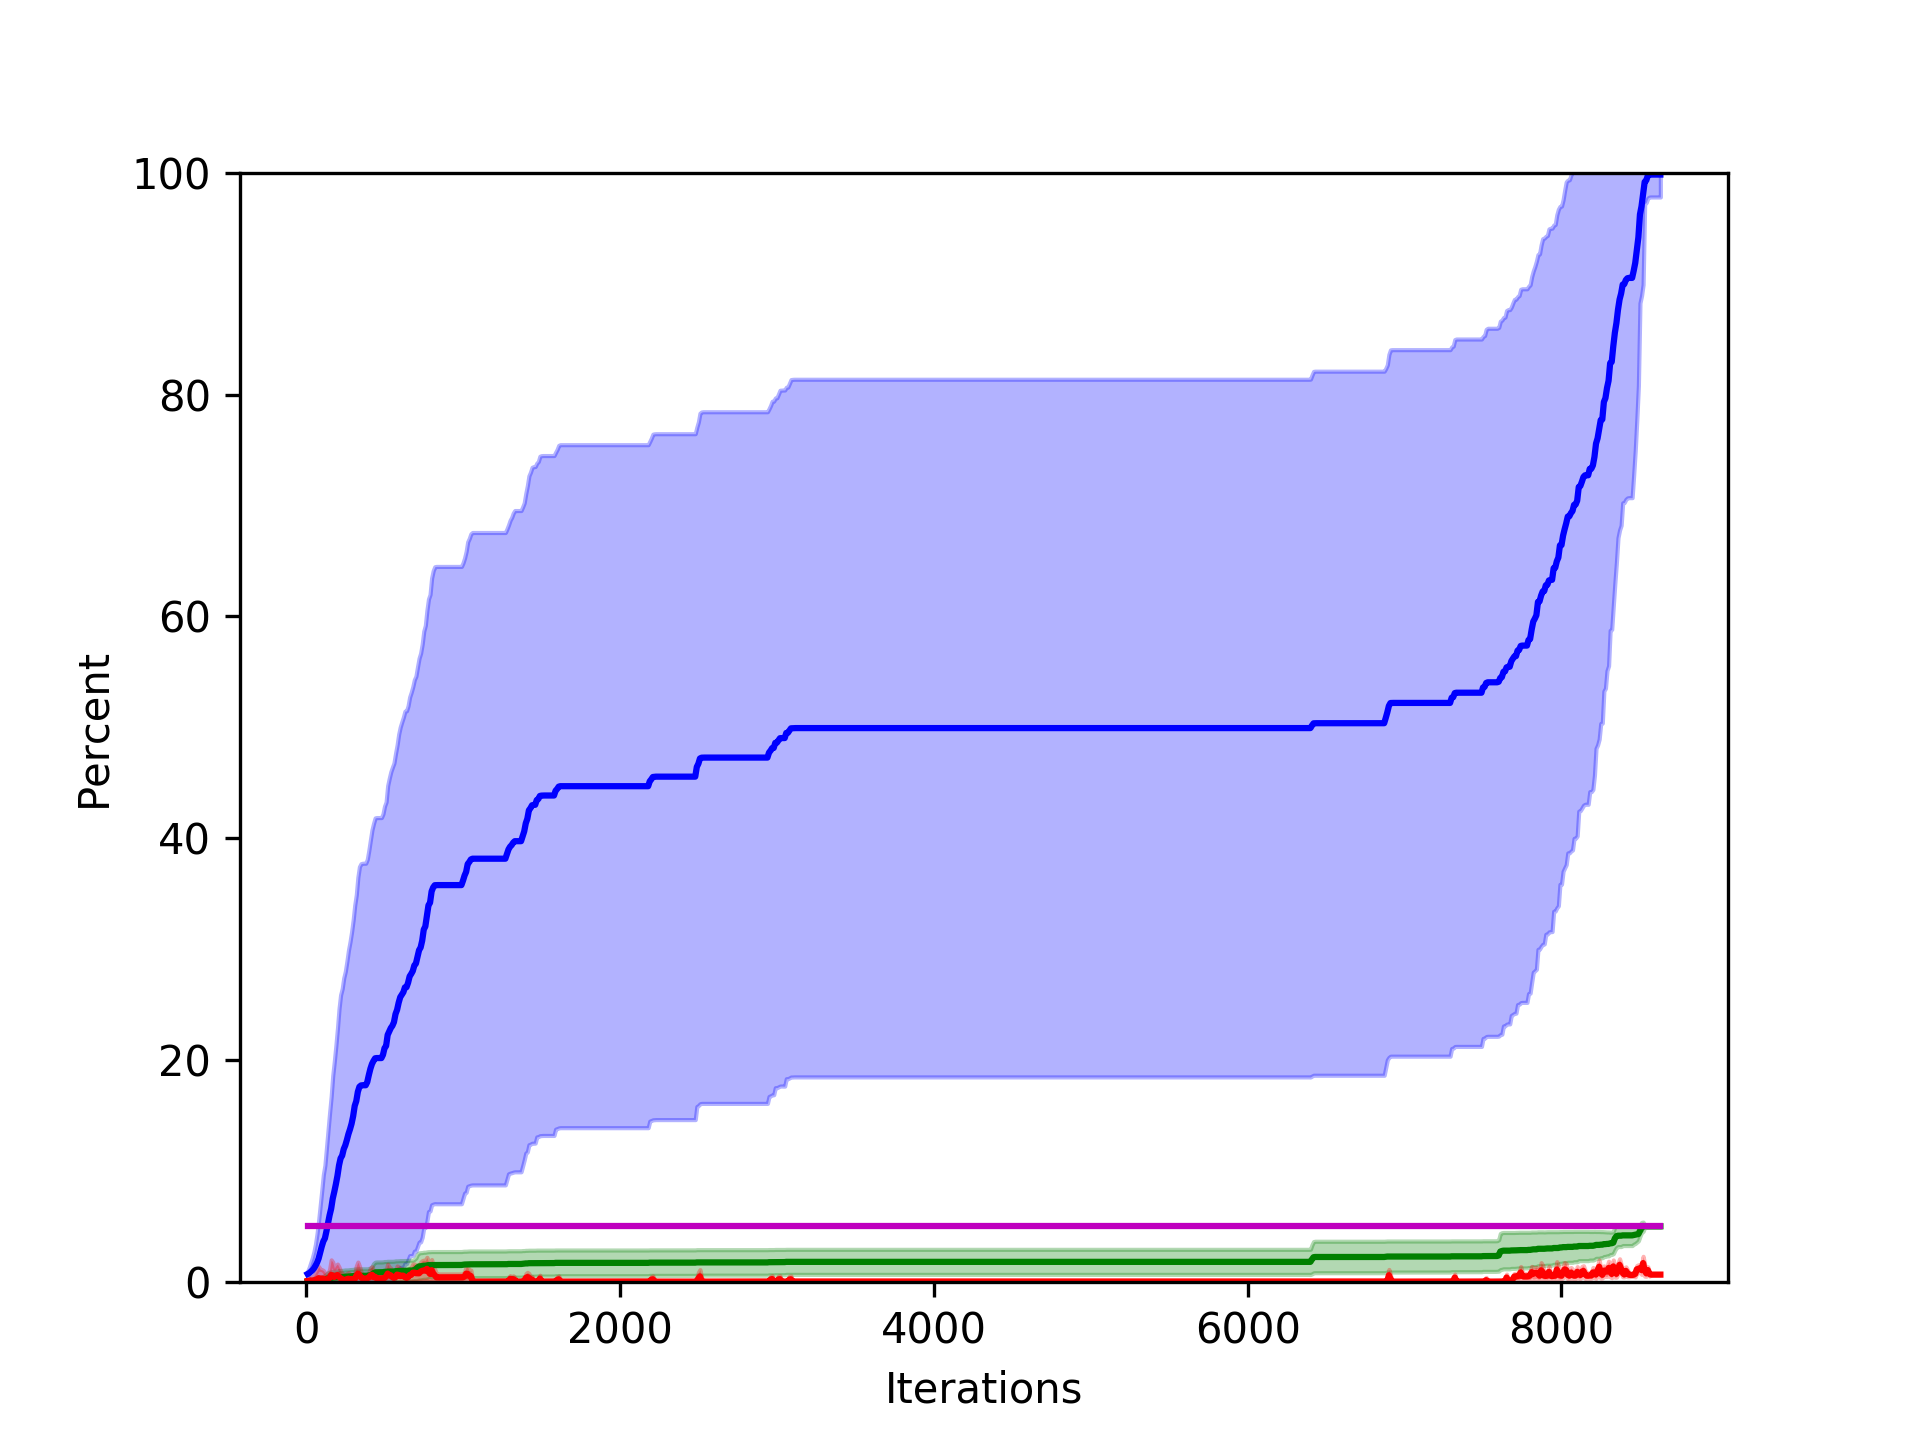
\includegraphics[width=\linewidth]{images/plots/Network_rA/10_5.png}
\caption{5\% malicious.}
\end{subfigure}

\vspace{1cm}

\begin{subfigure}{0.45\textwidth}
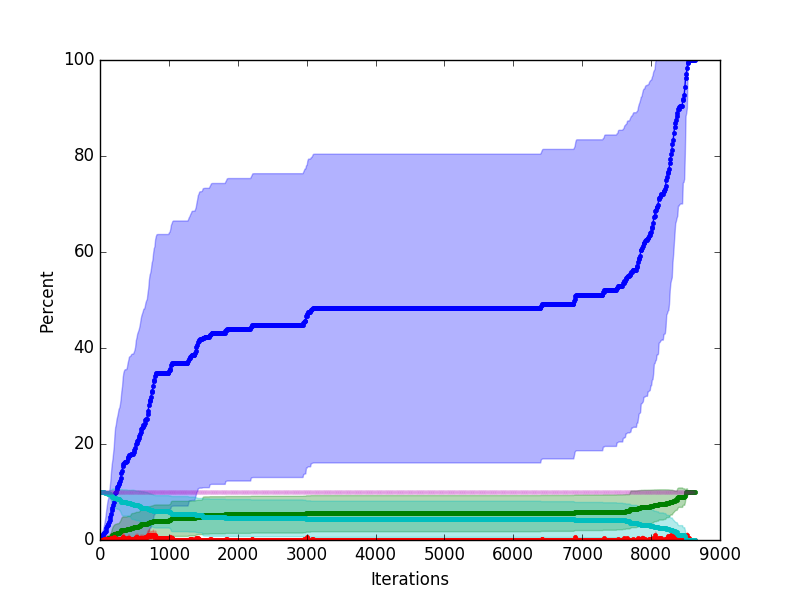
\includegraphics[width=\linewidth]{images/plots/Network_rA/10_10.png}
\caption{10\% malicious.}
\end{subfigure}
\hspace*{0.1cm} % separation between the subfigures
\begin{subfigure}{0.45\textwidth}
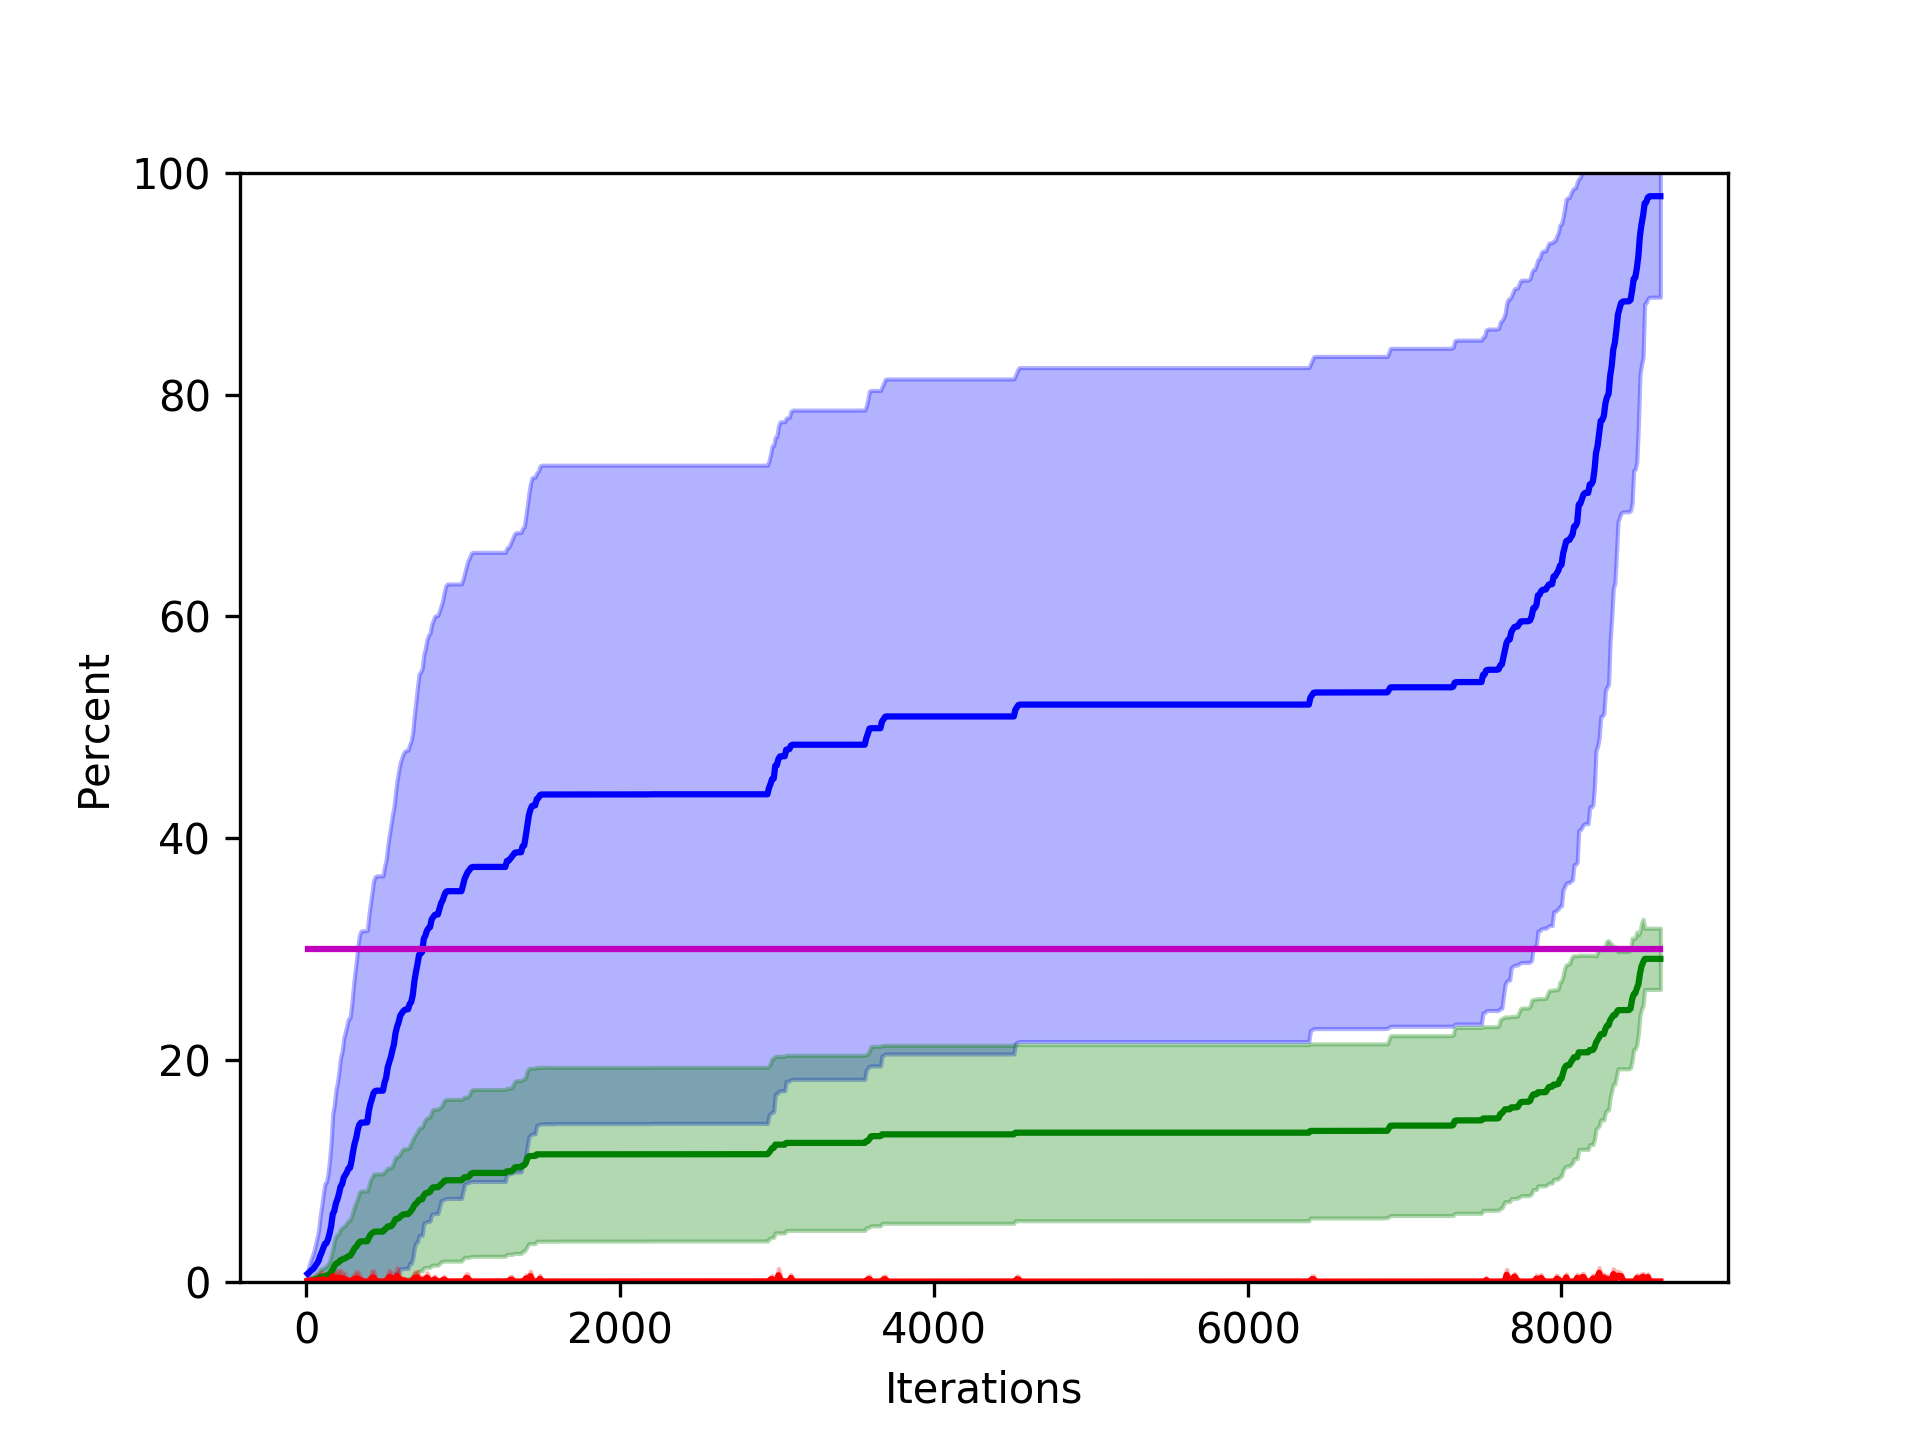
\includegraphics[width=\linewidth]{images/plots/Network_rA/10_30.png}
\caption{30\% malicious.}
\end{subfigure}

\vspace{1cm}

\begin{subfigure}{0.45\textwidth}
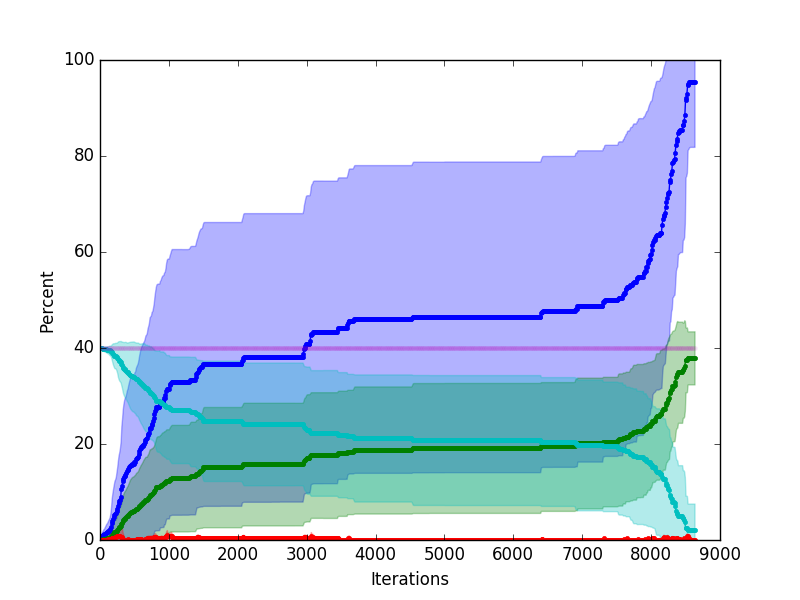
\includegraphics[width=\linewidth]{images/plots/Network_rA/10_40.png}
\caption{40\% malicious.}
\end{subfigure}
\hspace*{0.1cm} % separation between the subfigures
\begin{subfigure}{0.45\textwidth}
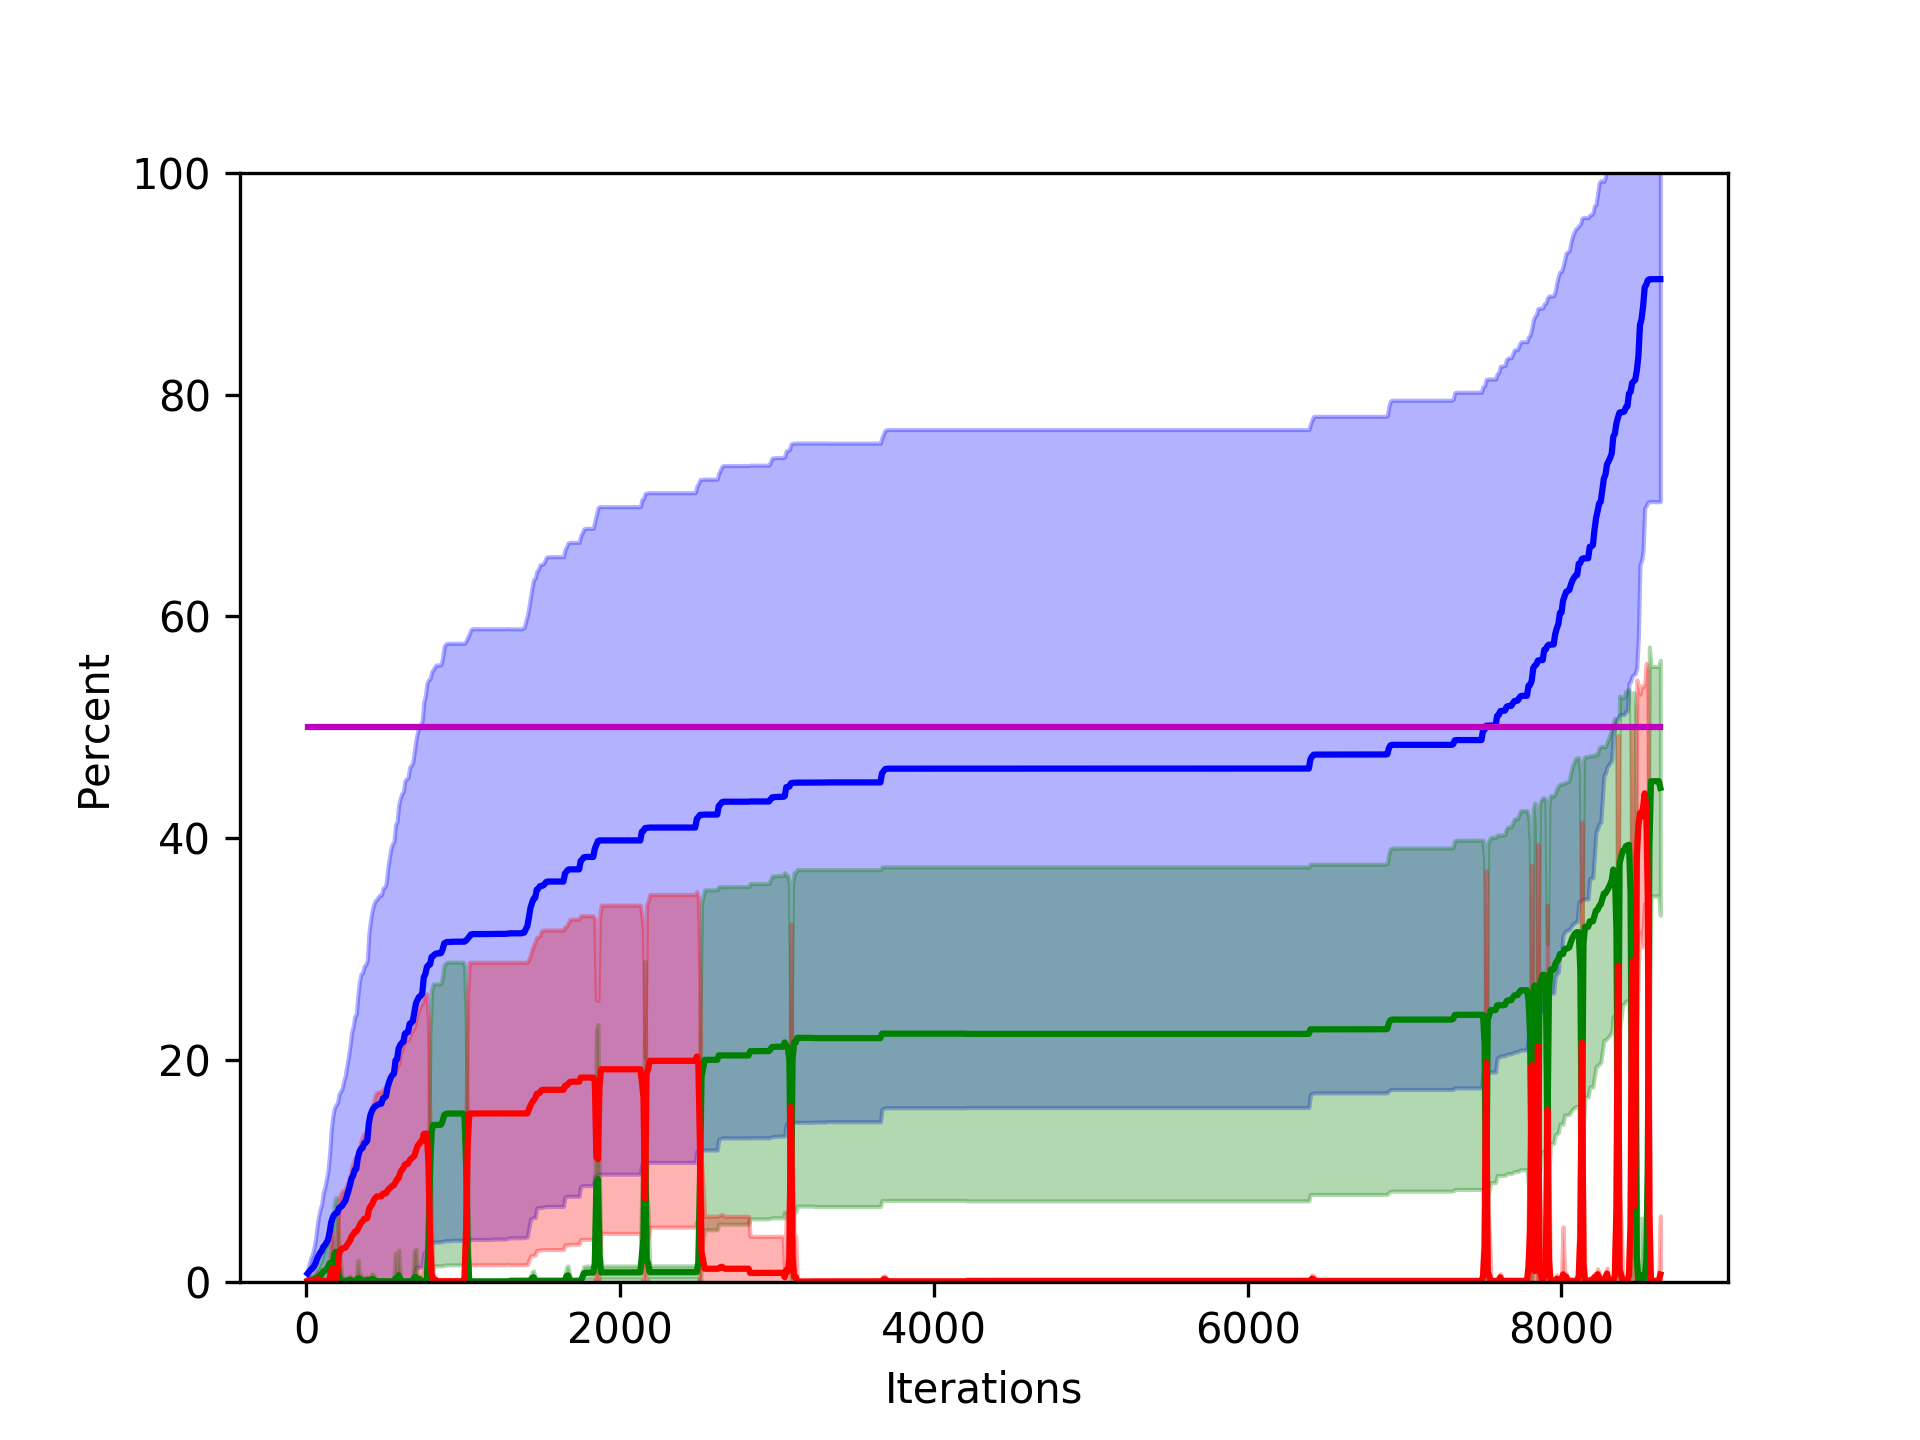
\includegraphics[width=\linewidth]{images/plots/Network_rA/10_50.png}
\caption{50\% malicious.}
\end{subfigure}


\caption{Simulation with $\rho$ = 10m and varying percentages of malicious nodes.}\label{fig:tarjan}
\end{figure}

\begin{figure}
\centering
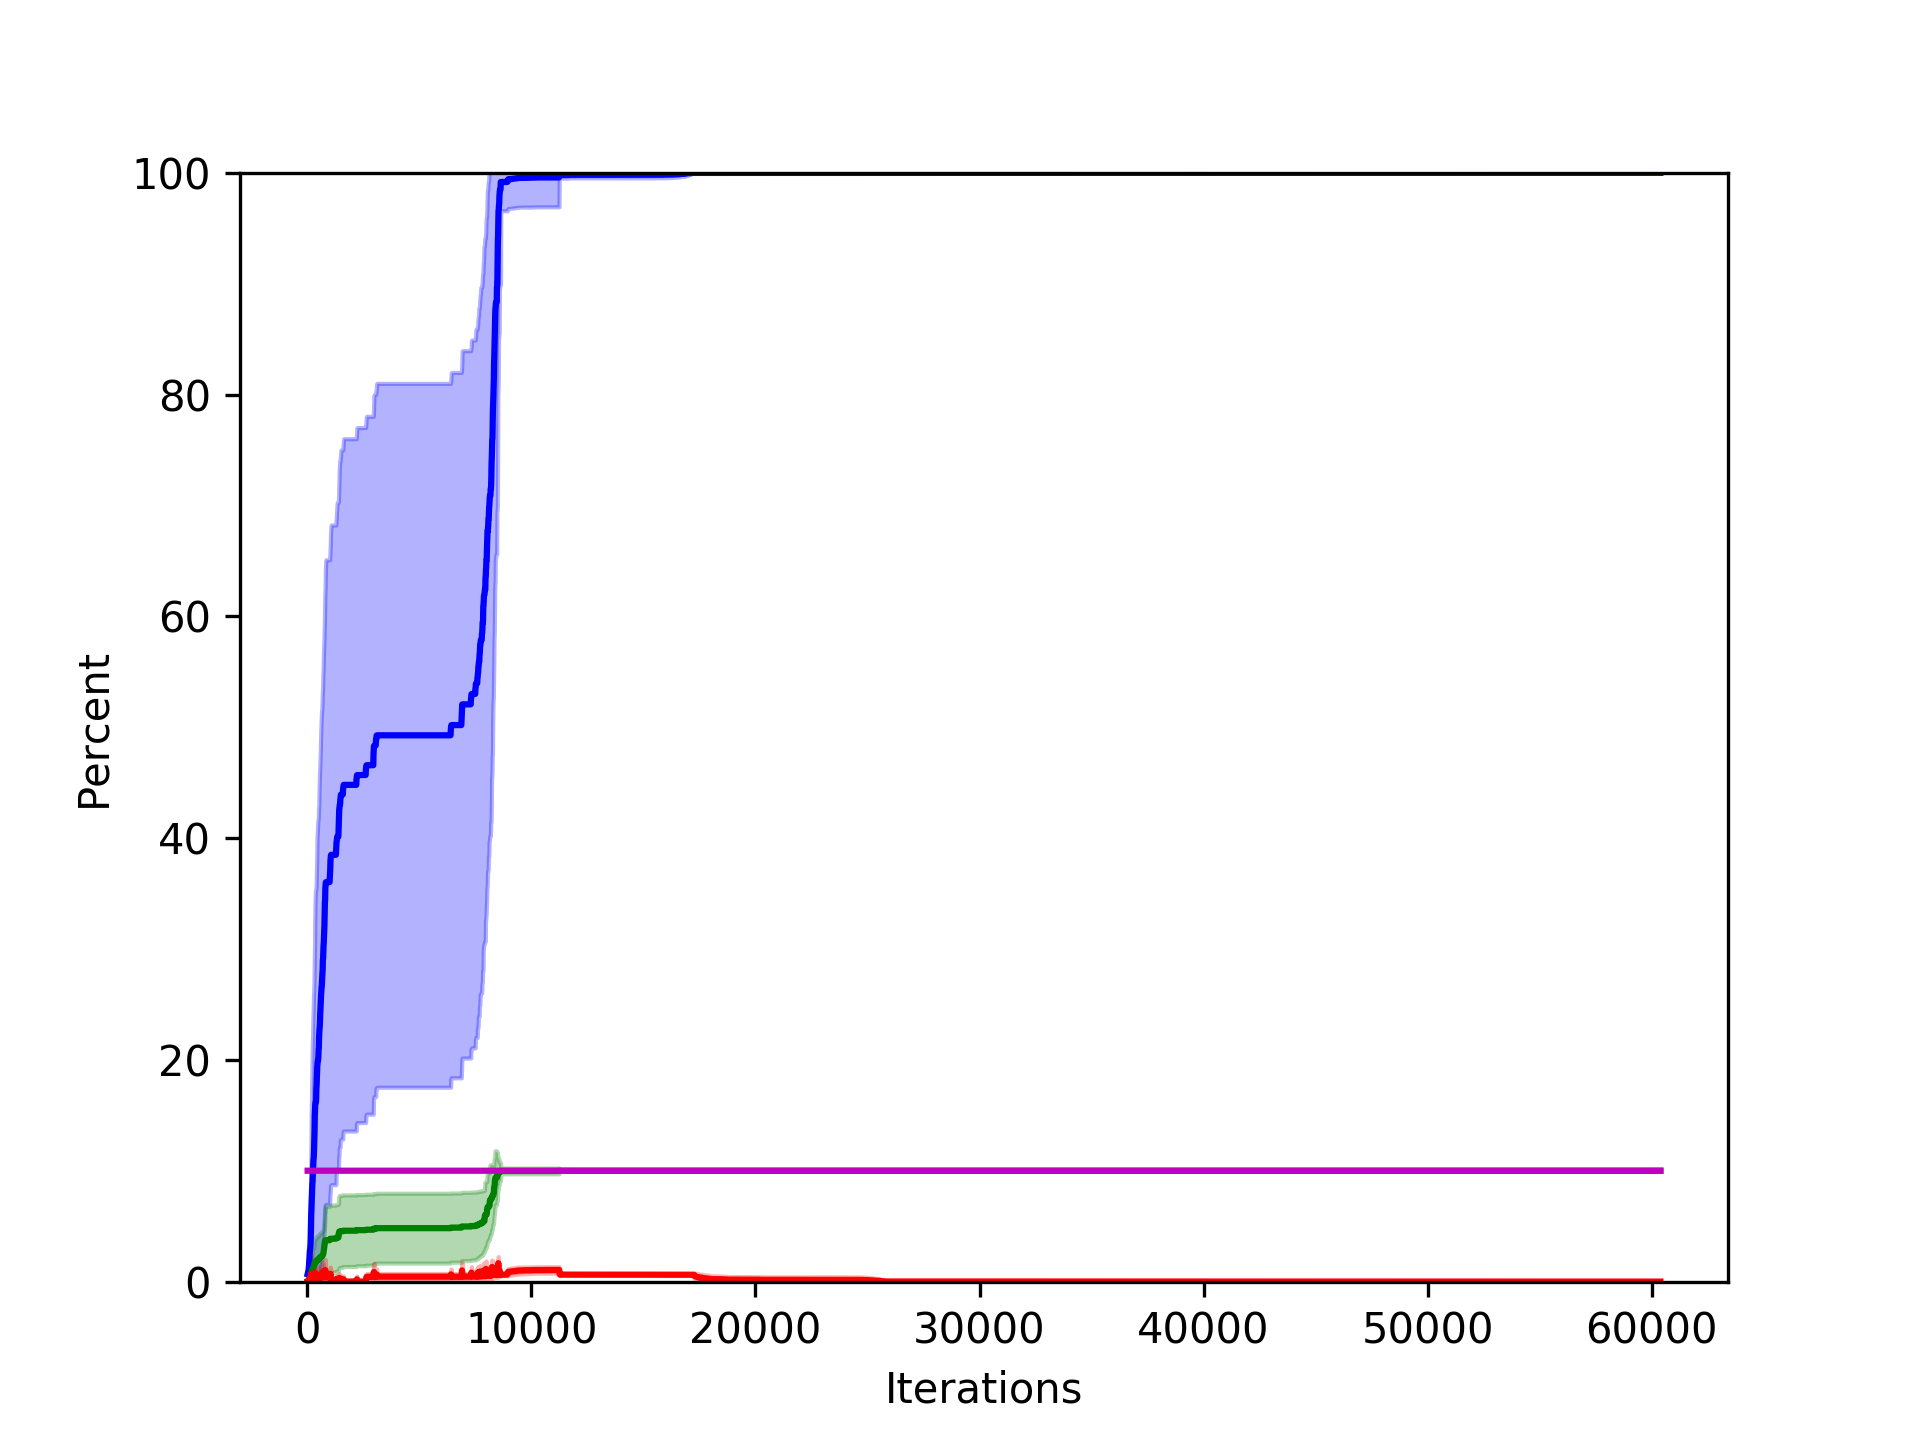
\includegraphics[width=0.5\textwidth]{images/plots/Network_rA7/10_10}
\caption{7 days scenario: 10m range and 10\% malicious nodes.} \label{fig:random7}
\end{figure}

%\begin{figure}
%\centering
%
%\begin{subfigure}{0.4\textwidth}
%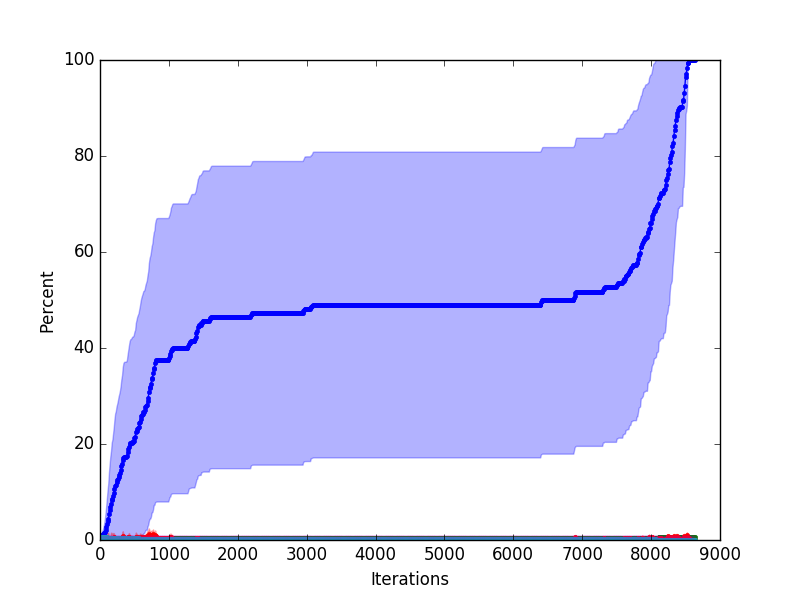
\includegraphics[width=\linewidth]{images/plots/Network_rA/10_1.png}
%\caption{1\% malicious.} \label{fig:tarjan0}
%\end{subfigure}
%
%\hspace*{1cm}
%
%\begin{subfigure}{0.4\textwidth}
%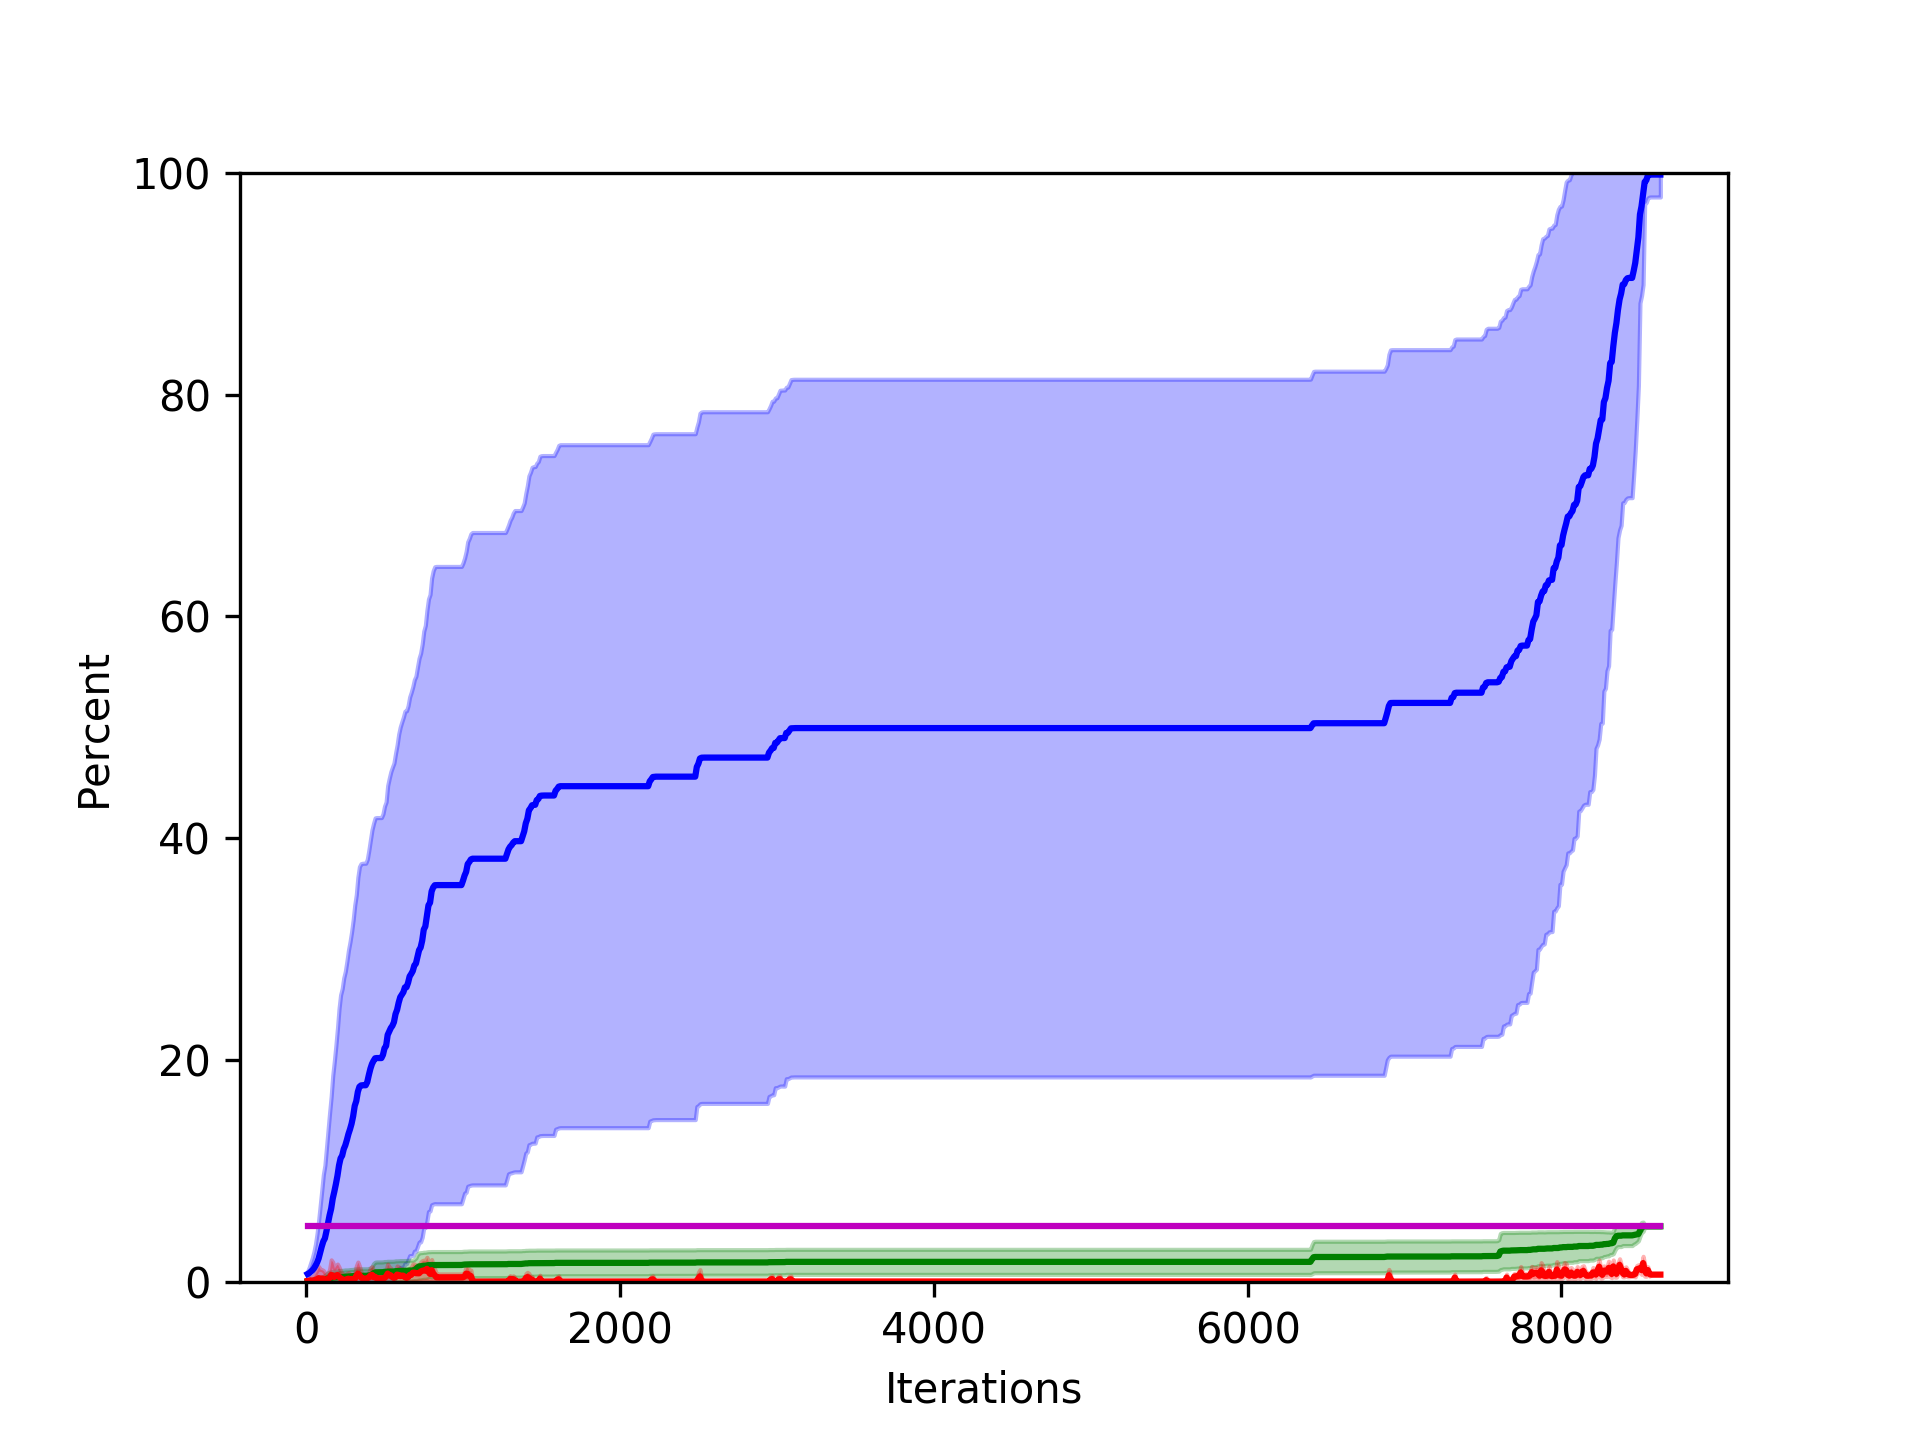
\includegraphics[width=\linewidth]{images/plots/Network_rA/10_5.png}
%\caption{5\% malicious.} \label{fig:tarjan0}
%\end{subfigure}
%
%\vspace{1cm}
%
%\begin{subfigure}{0.5\textwidth}
%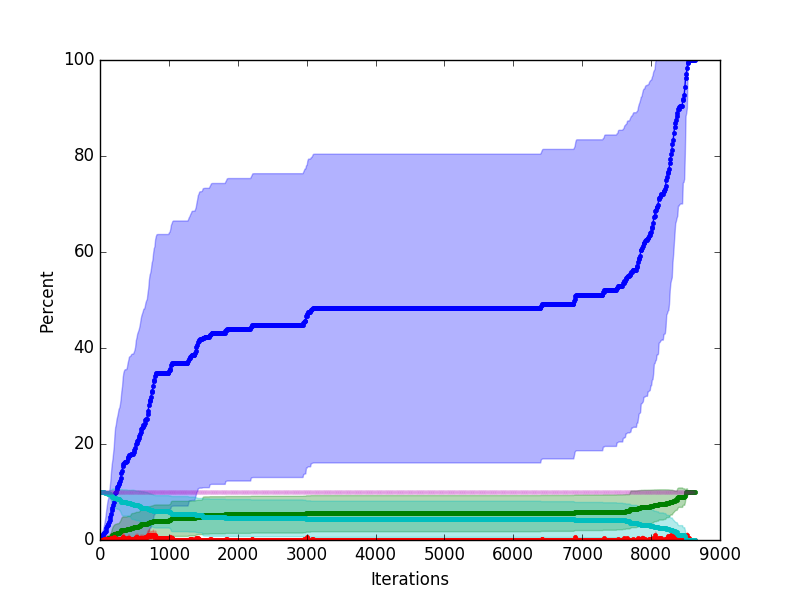
\includegraphics[width=\linewidth]{images/plots/Network_rA/10_10}
%\caption{10\% malicious.} \label{fig:tarjan0}
%\end{subfigure}
%
%\hspace*{\fill}
%
%\begin{subfigure}{0.5\textwidth}
%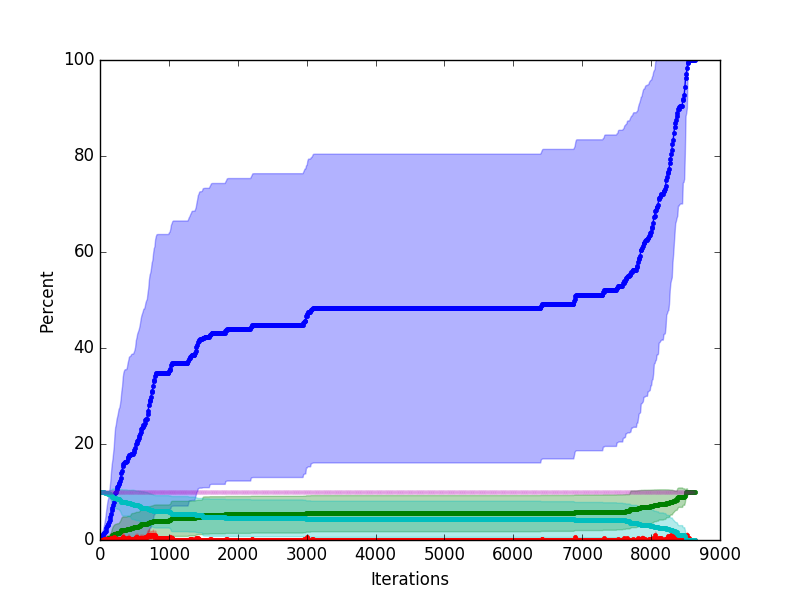
\includegraphics[width=\linewidth]{images/plots/Network_rA/10_10}
%\caption{$\rho$ = 50m.} \label{fig:tarjan0}
%\end{subfigure}
%
%\vspace{1cm}
%
%\begin{subfigure}{0.5\textwidth}
%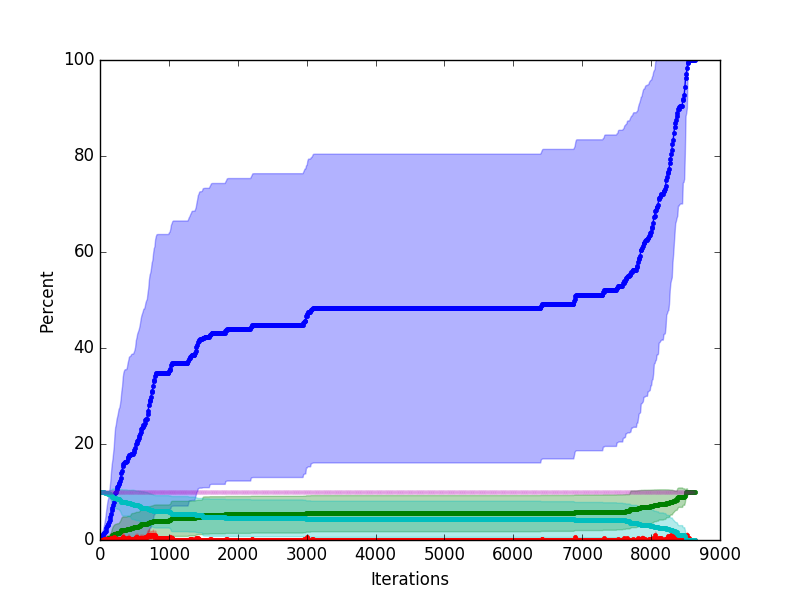
\includegraphics[width=\linewidth]{images/plots/Network_rA/10_10}
%\caption{$\rho$ = 50m.} \label{fig:tarjan0}
%\end{subfigure}
%
%\hspace*{\fill}
%
%\begin{subfigure}{0.5\textwidth}
%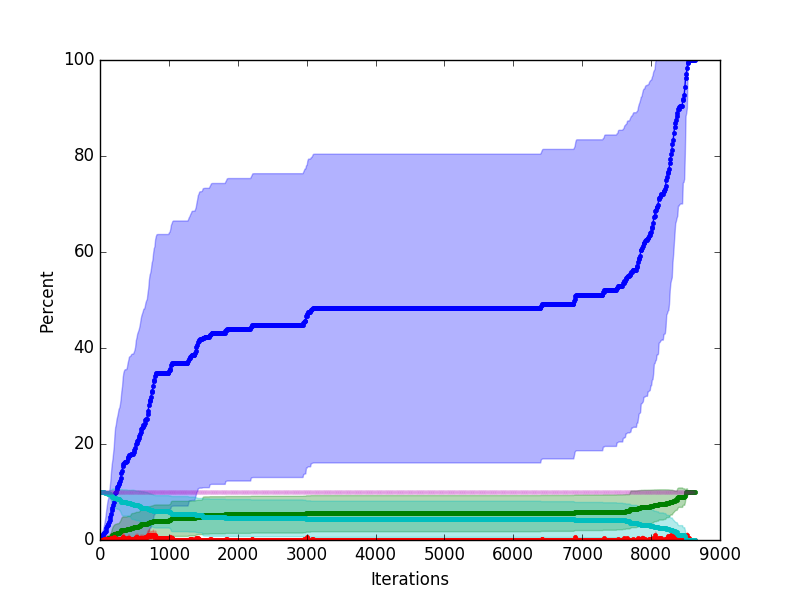
\includegraphics[width=\linewidth]{images/plots/Network_rA/10_10}
%\caption{$\rho$ = 50m.} \label{fig:tarjan0}
%\end{subfigure}
%
%\caption{Simulation with $\rho$ = 10m varying malicious.}
%\label{fig:random0}
%\end{figure}

%\begin{figure*}[!t]
%\centering
%\subfloat[]{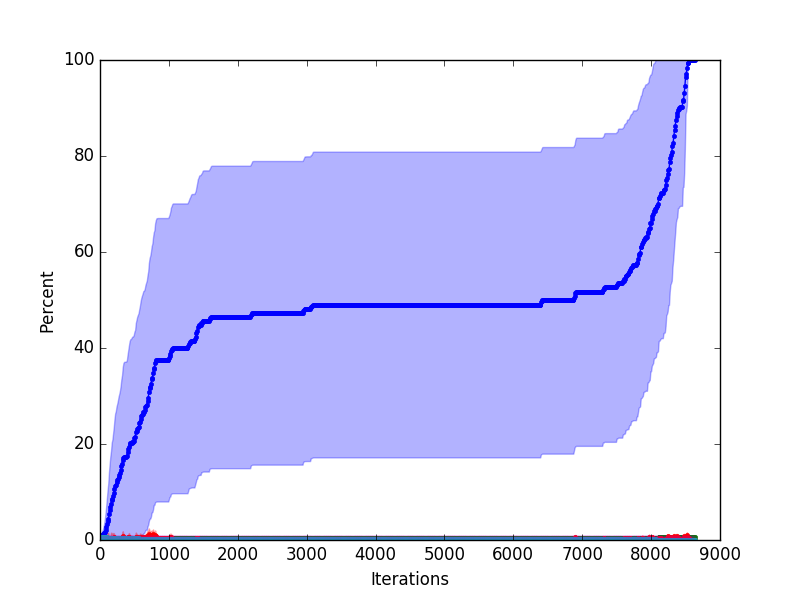
\includegraphics[width=0.329\linewidth]{images/plots/Network_rA/10_1}%
%\label{subfig:random1}}
%\hfil
%\subfloat[]{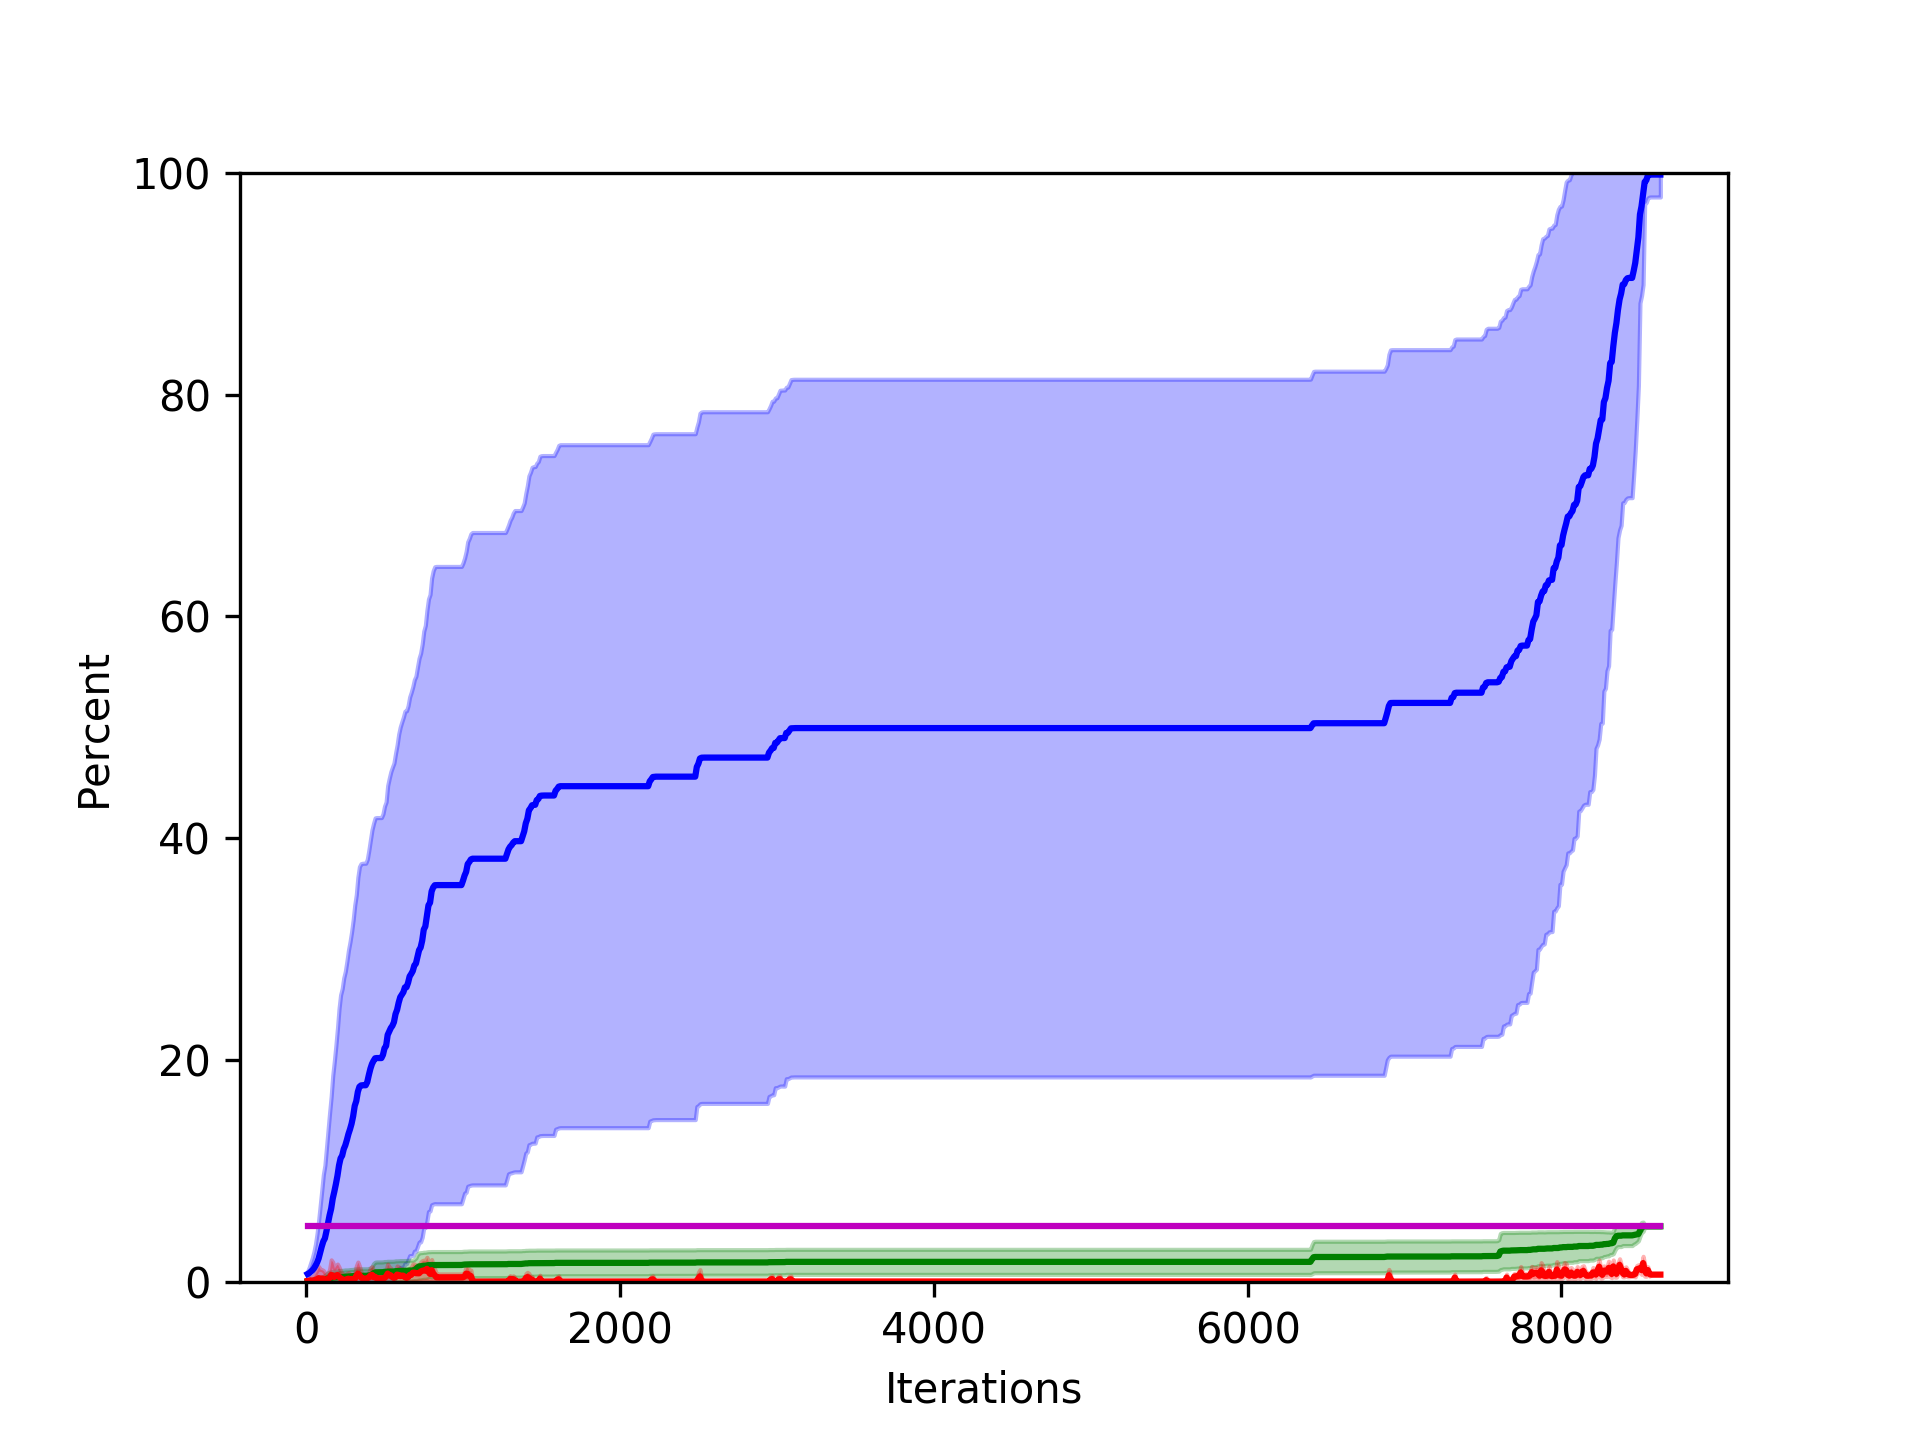
\includegraphics[width=0.329\linewidth]{images/plots/Network_rA/10_5}%
%\label{subfig:random2}}
%\hfil
%\subfloat[]{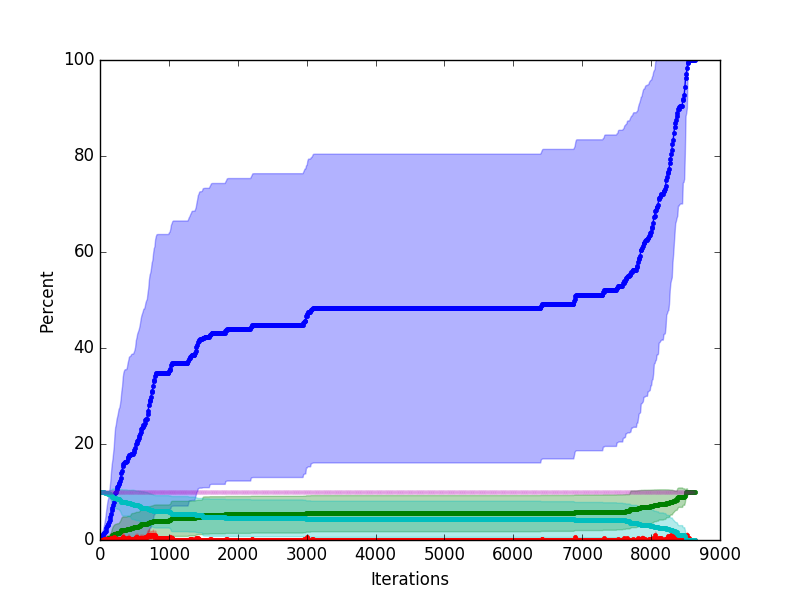
\includegraphics[width=0.329\linewidth]{images/plots/Network_rA/10_10}%
%\label{subfig:random3}}
%
%\subfloat[]{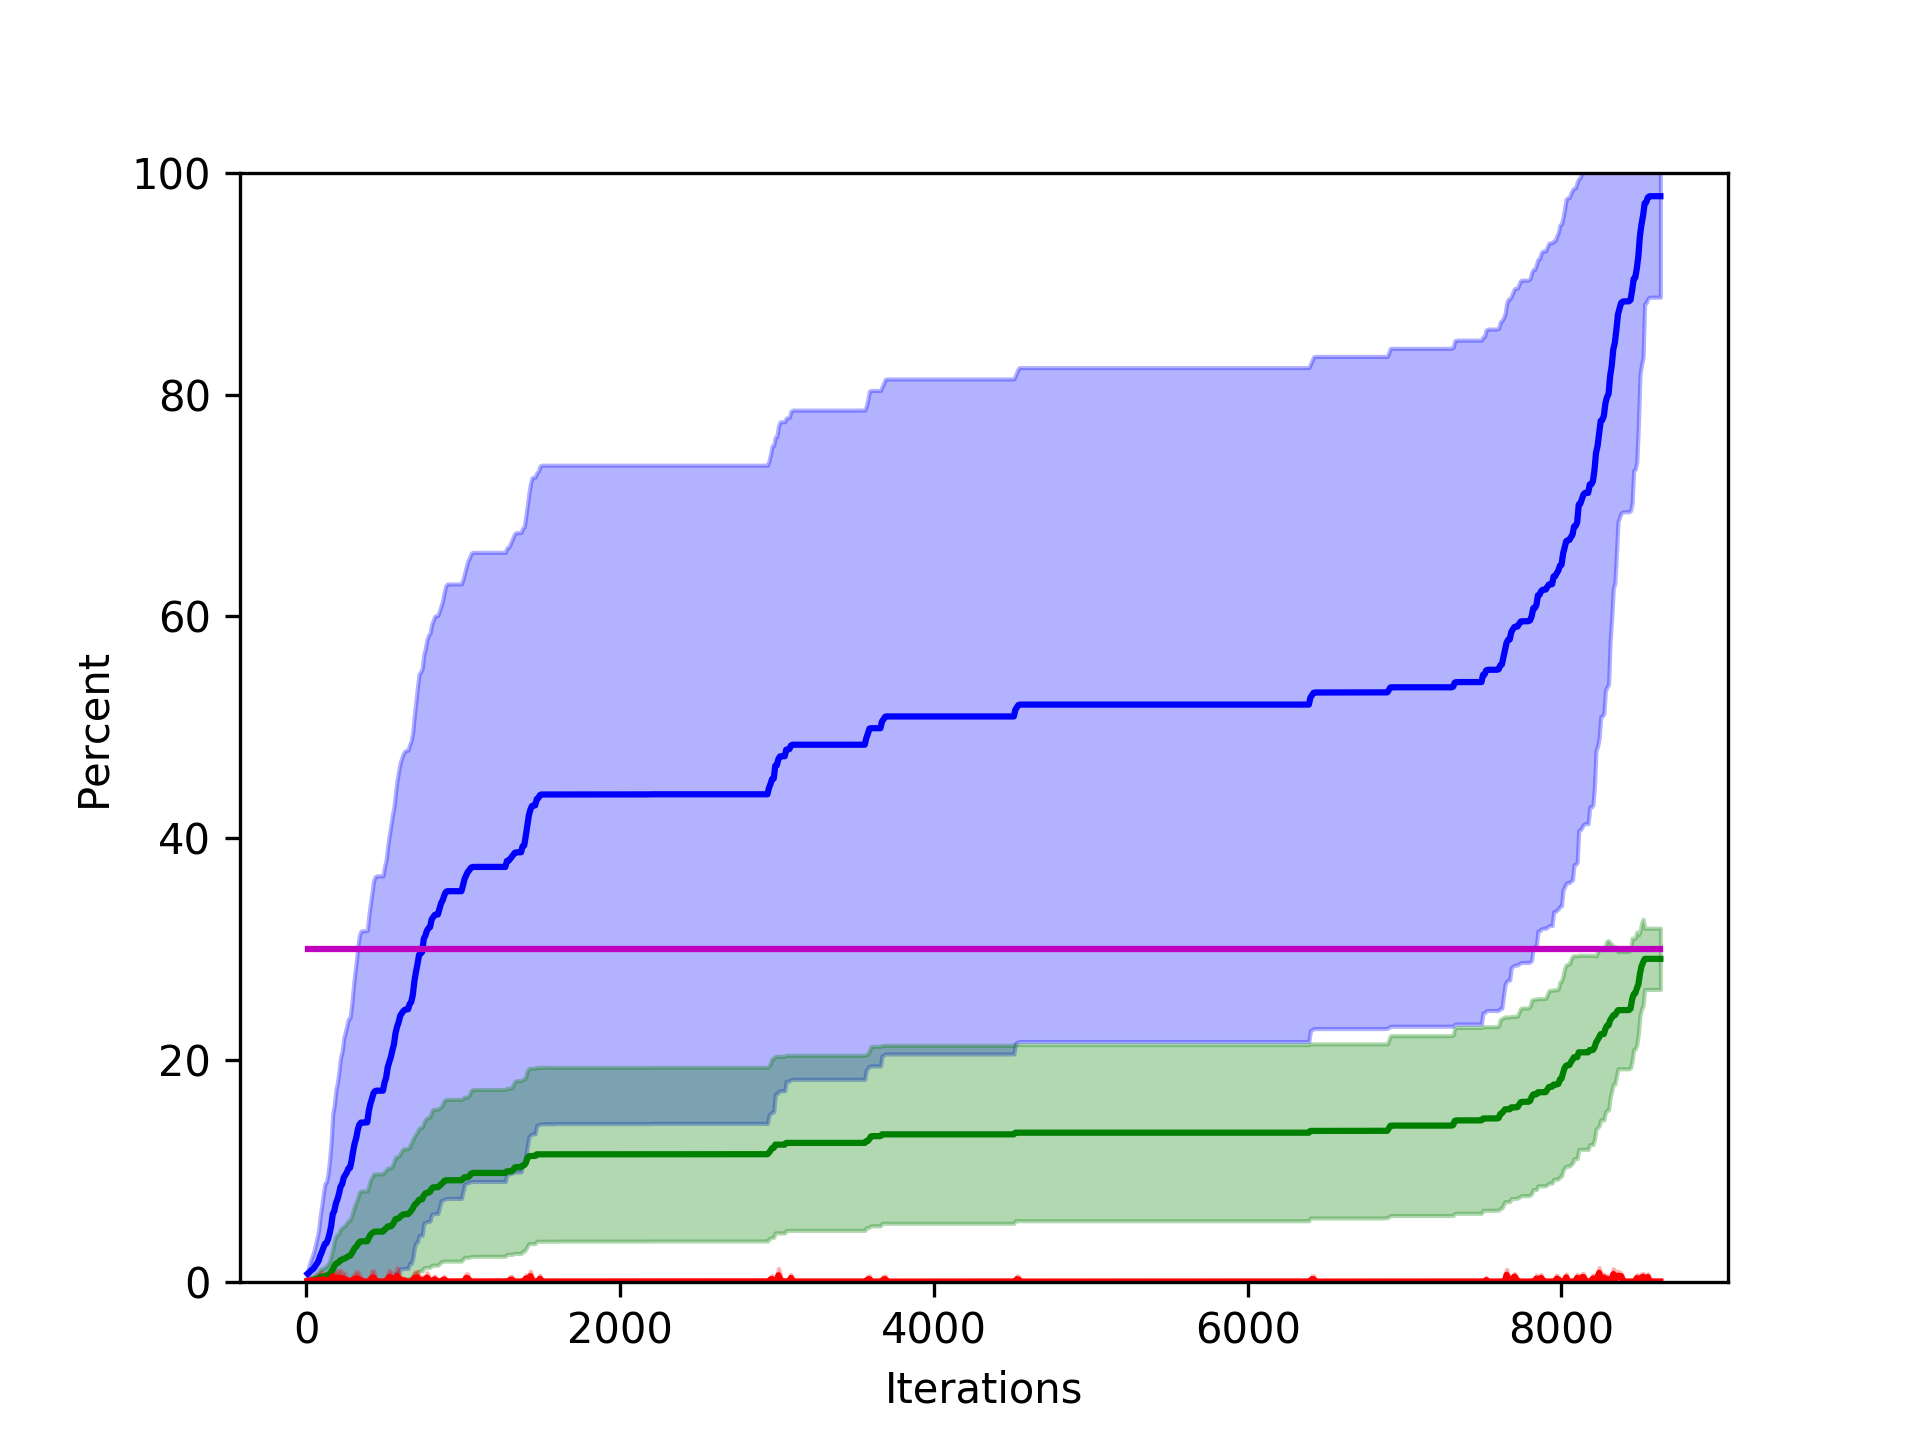
\includegraphics[width=0.329\linewidth]{images/plots/Network_rA/10_30}%
%\label{subfig:random4}}
%\hfil
%\subfloat[]{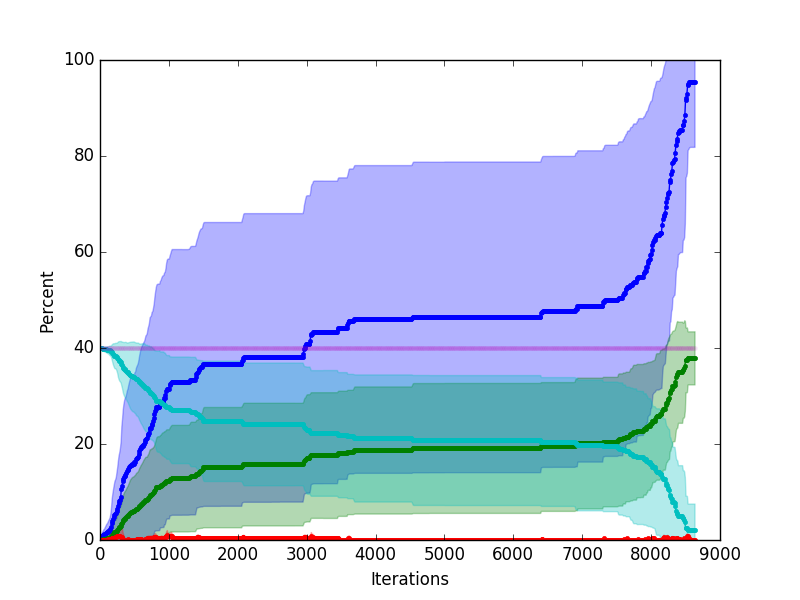
\includegraphics[width=0.329\linewidth]{images/plots/Network_rA/10_40}%
%\label{subfig:random5}}
%\hfil
%\subfloat[]{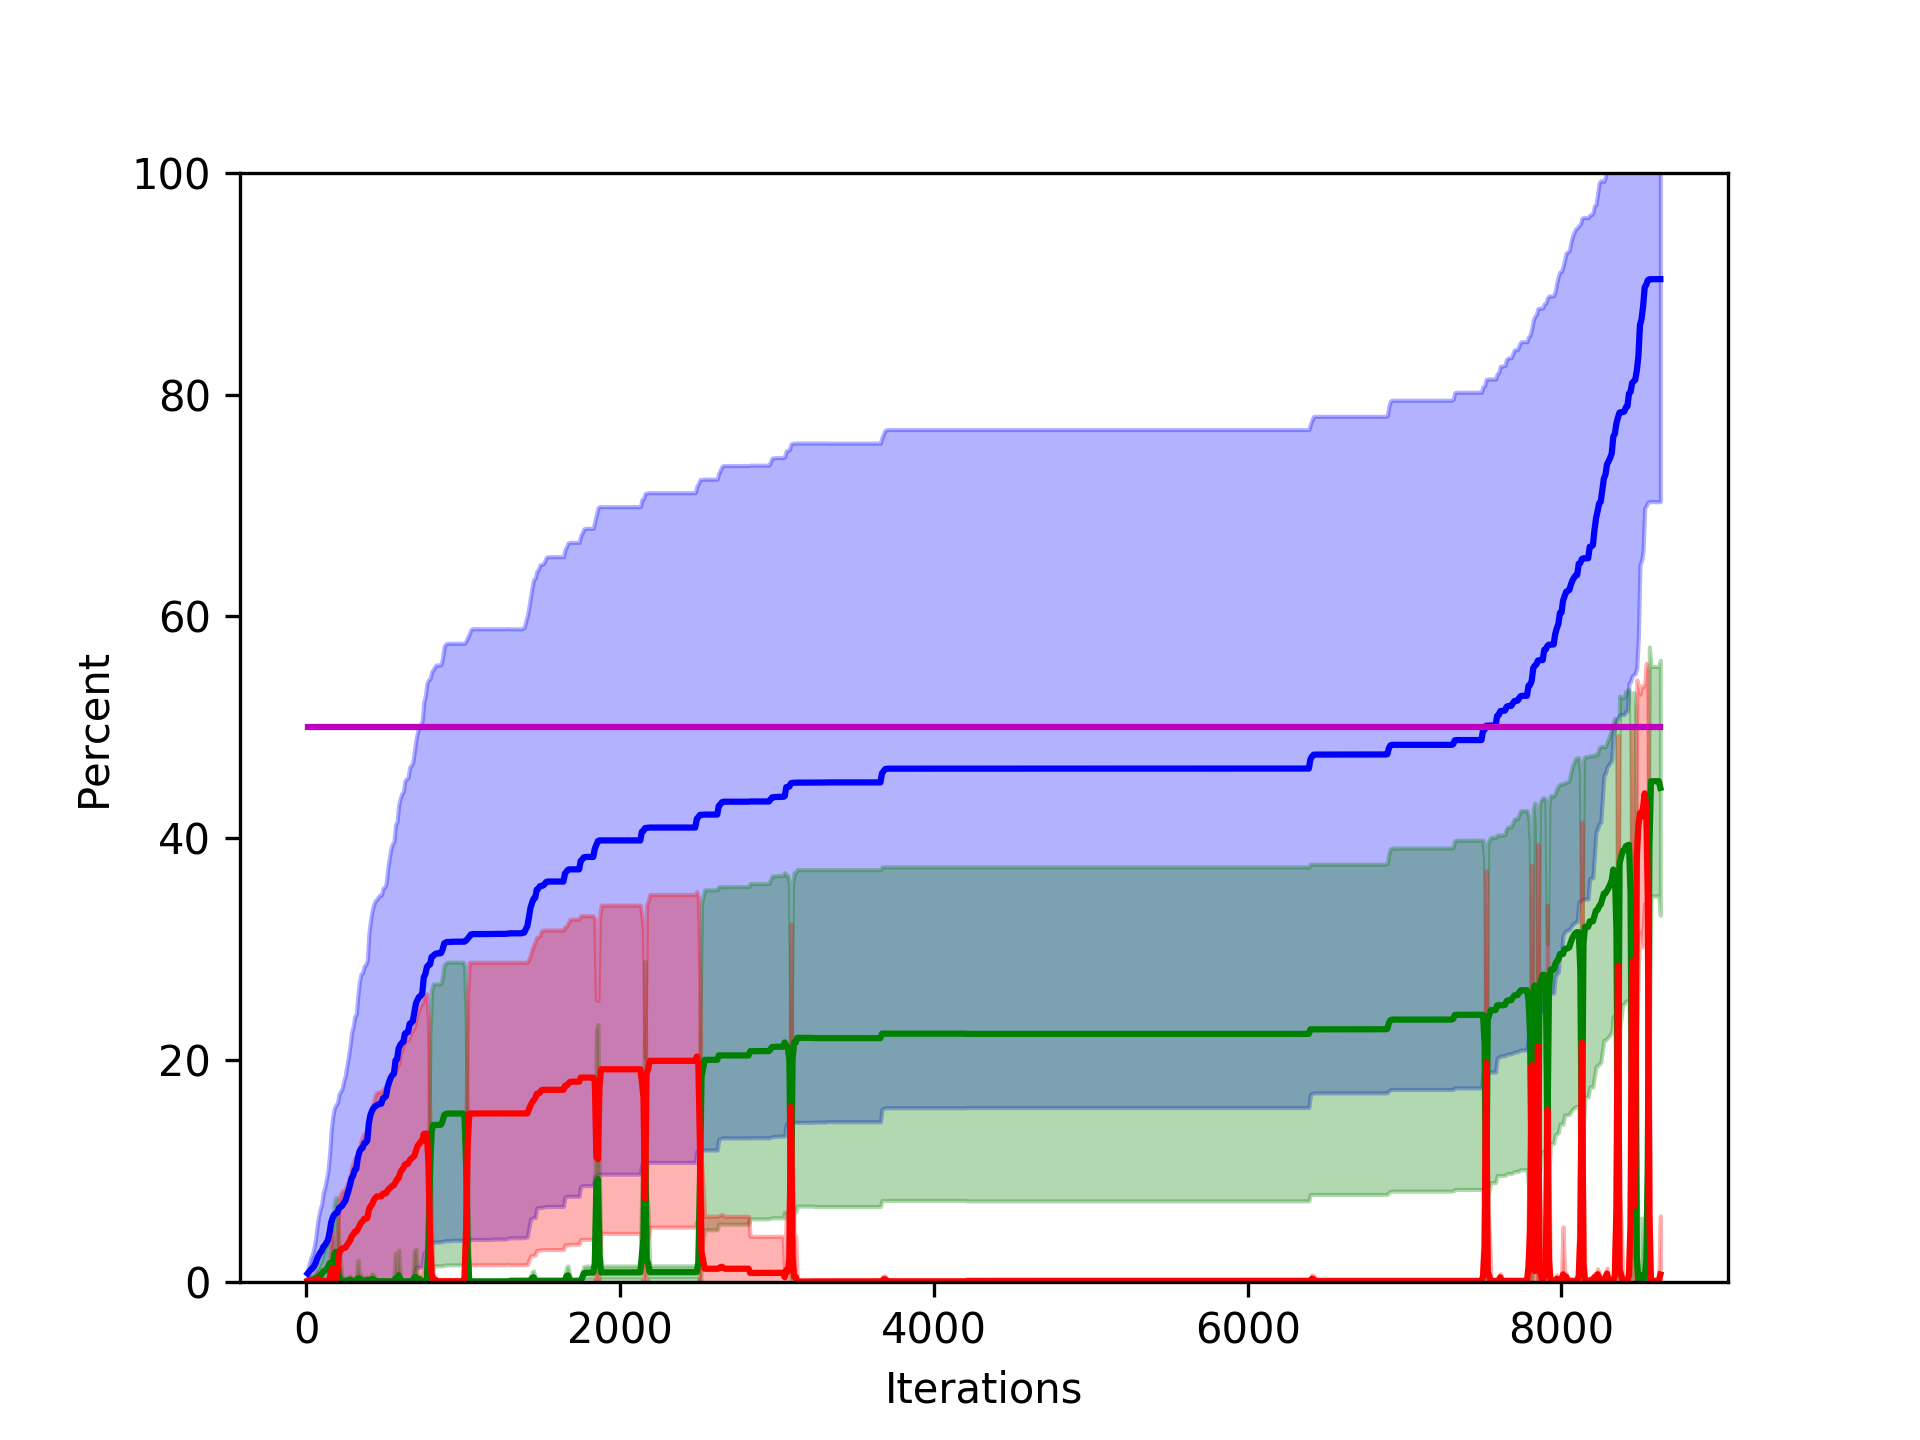
\includegraphics[width=0.329\linewidth]{images/plots/Network_rA/10_50}%
%\label{subfig:random6}}
%
%\caption{Simulation with $\rho$ = 10m and (a) 1\%, (b) 5\%, (c) 10\%, (d) 30\%, (e) 40\% or (f) 50\% malicious.}
%\label{fig:random0}
%\end{figure*}
